\documentclass{article}
\usepackage{graphicx} % Required for inserting images
\usepackage{enumitem}
\usepackage{xcolor}

\setlength{\oddsidemargin}{-0.25in}
\setlength{\topmargin}{-0.5in}
\setlength{\headheight}{0cm}
\setlength{\headsep}{0cm}
\setlength{\textheight}{10in}
\setlength{\textwidth}{7in}
\setlength{\topskip}{0cm}

\begin{document}

\noindent\textbf{ComS 472 - PS2 \quad Due: Sept 22, 2024 \quad Name: Aren Ashlock}

\begin{enumerate}

% ------------------------------------- 1 DONE -------------------------------------

\item \textbf{(12 pts)} (Exercise 3.17) Which of the following are true and which are false? Explain your answers.

    \begin{enumerate}[label=($\alph*$)]
    
    % ----------------------------------- 1a DONE -----------------------------------
    
    \item \textbf{(3 pts)} Depth-first search always expands at least as many nodes as A* search with an admissible heuristic.

    \color{blue}
        \textbf{False}, because A* is set at finding the optimal solution. Whereas, DFS may go down a branch that is non-optimal and have less node than the path A* finds. Thus, it may not always expand at least as many making the statement false.
    \color{black}

    % -------------------------------------------------------------------------------

    % ----------------------------------- 1b DONE -----------------------------------

    \item \textbf{(3 pts)} $h(n) = 0$ is an admissible heuristic for the 8-puzzle.

    \color{blue}
        \textbf{True}. This is because an admissible heuristic can never overestimate the cost to reach a goal. Since the actual cost is always $\geq 0$, it can never overestimate making the statement true.
    \color{black}\addtocounter{enumii}{1}

    % -------------------------------------------------------------------------------

    % ----------------------------------- 1d DONE -----------------------------------

    \item \textbf{(3 pts)} Breadth-first search is complete even if zero step costs are allowed.

    \color{blue}
        \textbf{True}, because the BFS is always complete since it explores every node at each level. Introducing zero step costs has no impact on the completeness.
    \color{black}

    % -------------------------------------------------------------------------------

    % ----------------------------------- 1e DONE -----------------------------------
    \item \textbf{(3 pts)} Assume that a rook can move on a chessboard any number of squares in a straight line, vertically or horizontally, but cannot jump over other pieces. Manhattan distance is an admissible heuristic for the problem of moving the rook from square A to square B in the smallest number of moves.

    \color{blue}
        \textbf{False}. My reasoning is that say the rook is in the bottom left corner and wants to move to the top right corner. If there are no pieces between those squares, it can be moved there in 1 move. However, the Manhattan distance would estimate however long the board is, which is likely > 1. Therefore, the statement is false.
    \color{black}

    % -------------------------------------------------------------------------------
    
    \end{enumerate}

% ----------------------------------------------------------------------------------

% ------------------------------------- 2 DONE -------------------------------------

\item \textbf{(10 pts)} (Exercise 3.18) Consider a state space where the start state is number 1 and each state $k$ has two successors: numbers $2k$ and $2k + 1$.

\begin{enumerate}[label=($\alph*$)]
    
    % ----------------------------------- 2a DONE -----------------------------------
    
    \item \textbf{(4 pts)} Draw the portion of the state space for states 1 to 15.

    \color{blue}
        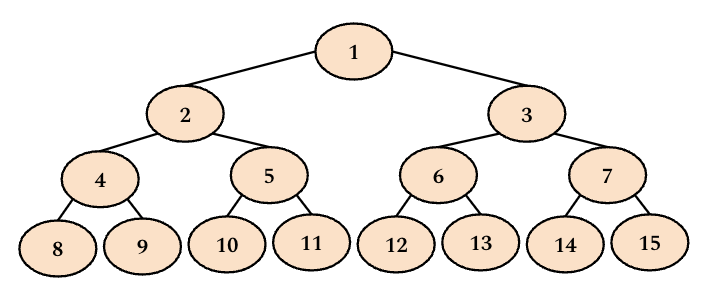
\includegraphics[scale=0.5]{472-PS2-Q2A.png}
    \color{black}

    % -------------------------------------------------------------------------------

    % ----------------------------------- 2b DONE -----------------------------------

    \item \textbf{(6 pts)} Suppose the goal state is 11. List the order in which nodes will be visited for breadth-first search, depth-limited search with limit 3, and iterative deepening search.

    \color{blue}
        \textbf{BFS}: 1, 2, 3, 4, 5, 6, 7, 8, 9, 10, 11\\
        \textbf{DLS}: 1, 2, 4, 8, 9, 5, 10, 11\\
        \textbf{IDS}: 1, 1, 2, 3, 1, 2, 4, 5, 3, 6, 7, 1, 2, 4, 8, 9, 5, 10, 11
    \color{black}

    % -------------------------------------------------------------------------------

    \end{enumerate}

% ----------------------------------------------------------------------------------

% ------------------------------------- 3 DONE -------------------------------------

\item \textbf{(5 pts)} (Exercise 3.22) Describe a state space in which iterative deepening search performs much worse than depth-first search (for example, $O(n^2)$ vs. $O(n)$).

\color{blue}
    Say there are $n$ states and the branching factor is 1. DFS will perform $O(n)$ since it explores at worst $n$ nodes. However, IDS will perform $O(n^2)$ since in it's worst-case scenario, it expands $1+2+3+...+n$ node. This is equivalent to $\frac{n(n+1)}{2}$, which gives a performance of $O(n^2)$.
\color{black}

% ----------------------------------------------------------------------------------

% ------------------------------------- 4 DONE -------------------------------------

\item \textbf{(18 pts)} (Exercise 3.27) Trace the operation of A* search applied to the problem of getting to Bucharest from Lugoj using the straight-line distance heuristic. That is, show the sequence of nodes that the algorithm will consider and the $f$, $g$, and $h$ scores for each node.

    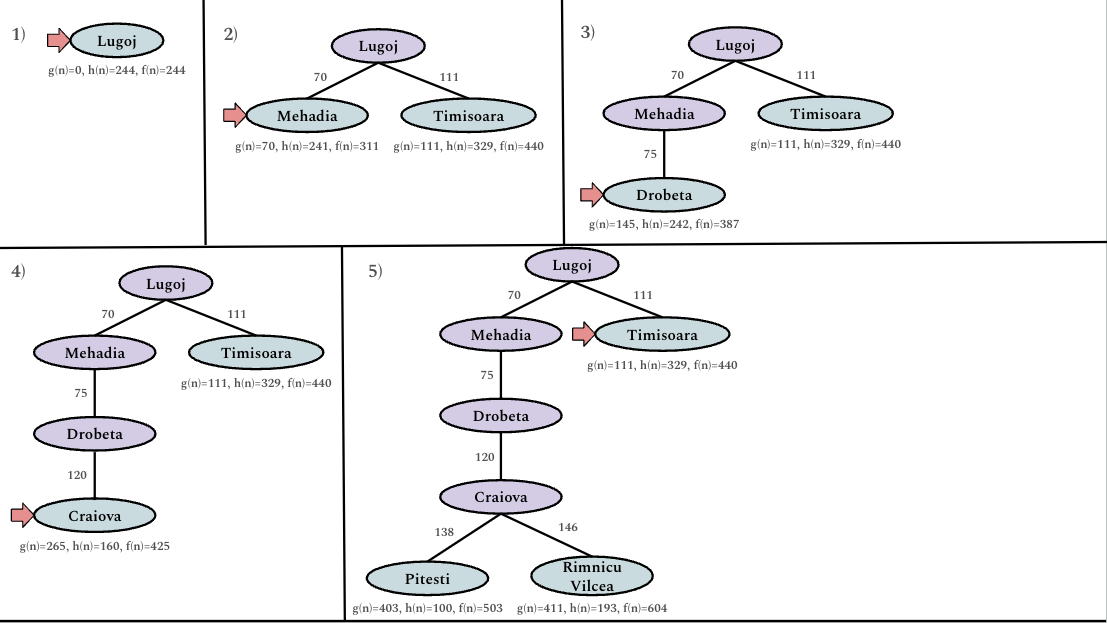
\includegraphics[scale=0.55]{472-PS2-Q4-1thru5.png}\\
    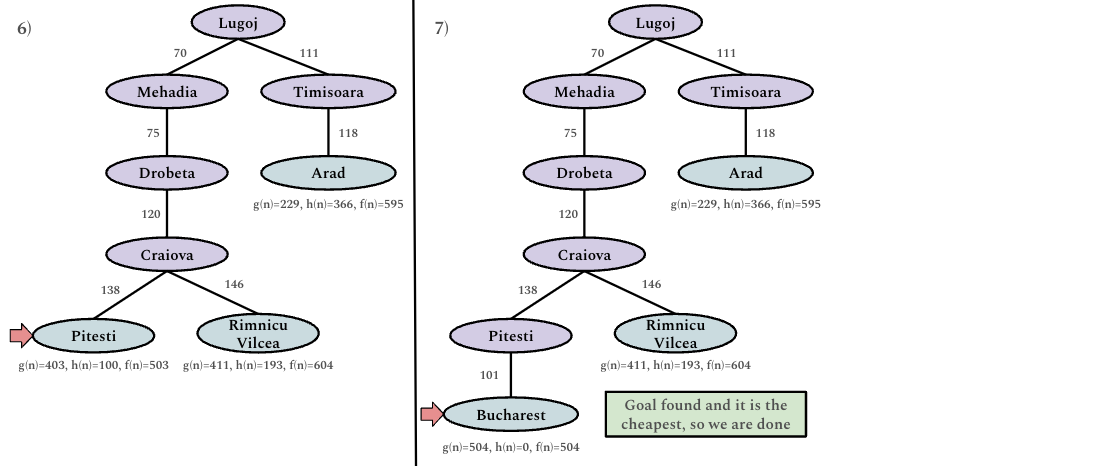
\includegraphics[scale=0.55]{472-PS2-Q4-6thru7.png}

% ----------------------------------------------------------------------------------

% ------------------------------------- 5 DONE -------------------------------------

\item \textbf{(10 pts)} (Exercise 3.31) The heuristic path algorithm is a best-first search in which the evaluation function is $f(n) = (2-w)g(n) + wh(n)$.

\begin{enumerate}[label=($\alph*$)]
    
    % ----------------------------------- 5a DONE -----------------------------------
    
    \item \textbf{(3 pts)} For what values of $w$ is this complete?

    \color{blue}
        $0 \leq w < 2$. We know that Greedy Best-First Search is not complete due to solely relying on the heuristic cost, it may not find a solution. However, for all other values, the cost to the node is considered and a solution will always be found (whether optimally or not).\\\\
    \color{black}

    % -------------------------------------------------------------------------------

    % ----------------------------------- 5b DONE -----------------------------------

    \item \textbf{(4 pts)} For what values is it optimal, assuming that $h$ is admissible?

    \color{blue}
        $0 \leq w \leq 1$. In this range it behaves closer to Uniform-Cost Search (when $w$ is closer to 0) or A* Search (when $w$ is closer to 1) which both are optimal. However, when $w > 1$, it behaves more like Greedy Best-First Search, which we know if not necessarily optimal since it only focuses on the heuristic to determine the path.
    \color{black}

    % -------------------------------------------------------------------------------

    % ----------------------------------- 5c DONE -----------------------------------

    \item \textbf{(3 pts)} What kind of search does this perform for $w=0$, $w=1$, and $w=2$?

    \color{blue}
        When $w = 0$, it performs \textbf{Uniform-Cost Search} since it ignores the heuristic and focuses on the actual cost to the node. For $w = 1$, it performs \textbf{A* Search} since it incorporates both the actual cost to the node and the heuristic. As for $w = 2$, it performs \textbf{Greedy Best-First Search} since it only factors in the heuristic.
    \color{black}

    % -------------------------------------------------------------------------------
    
    \end{enumerate}

% ----------------------------------------------------------------------------------

\end{enumerate}
\end{document}